% Options for packages loaded elsewhere
\PassOptionsToPackage{unicode}{hyperref}
\PassOptionsToPackage{hyphens}{url}
%
\documentclass[
]{article}
\usepackage[russian]{babel}
\usepackage{amsmath,amssymb}
\usepackage{lmodern}
\usepackage{iftex}
\ifPDFTeX
  \usepackage[T1]{fontenc}
  \usepackage[utf8]{inputenc}
  \usepackage{textcomp} % provide euro and other symbols
\else % if luatex or xetex
  \usepackage{unicode-math}
  \defaultfontfeatures{Scale=MatchLowercase}
  \defaultfontfeatures[\rmfamily]{Ligatures=TeX,Scale=1}
\fi
% Use upquote if available, for straight quotes in verbatim environments
\IfFileExists{upquote.sty}{\usepackage{upquote}}{}
\IfFileExists{microtype.sty}{% use microtype if available
  \usepackage[]{microtype}
  \UseMicrotypeSet[protrusion]{basicmath} % disable protrusion for tt fonts
}{}
\makeatletter
\@ifundefined{KOMAClassName}{% if non-KOMA class
  \IfFileExists{parskip.sty}{%
    \usepackage{parskip}
  }{% else
    \setlength{\parindent}{0pt}
    \setlength{\parskip}{6pt plus 2pt minus 1pt}}
}{% if KOMA class
  \KOMAoptions{parskip=half}}
\makeatother
\usepackage{xcolor}
\usepackage{color}
\usepackage{fancyvrb}
\newcommand{\VerbBar}{|}
\newcommand{\VERB}{\Verb[commandchars=\\\{\}]}
\DefineVerbatimEnvironment{Highlighting}{Verbatim}{commandchars=\\\{\}}
% Add ',fontsize=\small' for more characters per line
\newenvironment{Shaded}{}{}
\newcommand{\AlertTok}[1]{\textcolor[rgb]{1.00,0.00,0.00}{\textbf{#1}}}
\newcommand{\AnnotationTok}[1]{\textcolor[rgb]{0.38,0.63,0.69}{\textbf{\textit{#1}}}}
\newcommand{\AttributeTok}[1]{\textcolor[rgb]{0.49,0.56,0.16}{#1}}
\newcommand{\BaseNTok}[1]{\textcolor[rgb]{0.25,0.63,0.44}{#1}}
\newcommand{\BuiltInTok}[1]{\textcolor[rgb]{0.00,0.50,0.00}{#1}}
\newcommand{\CharTok}[1]{\textcolor[rgb]{0.25,0.44,0.63}{#1}}
\newcommand{\CommentTok}[1]{\textcolor[rgb]{0.38,0.63,0.69}{\textit{#1}}}
\newcommand{\CommentVarTok}[1]{\textcolor[rgb]{0.38,0.63,0.69}{\textbf{\textit{#1}}}}
\newcommand{\ConstantTok}[1]{\textcolor[rgb]{0.53,0.00,0.00}{#1}}
\newcommand{\ControlFlowTok}[1]{\textcolor[rgb]{0.00,0.44,0.13}{\textbf{#1}}}
\newcommand{\DataTypeTok}[1]{\textcolor[rgb]{0.56,0.13,0.00}{#1}}
\newcommand{\DecValTok}[1]{\textcolor[rgb]{0.25,0.63,0.44}{#1}}
\newcommand{\DocumentationTok}[1]{\textcolor[rgb]{0.73,0.13,0.13}{\textit{#1}}}
\newcommand{\ErrorTok}[1]{\textcolor[rgb]{1.00,0.00,0.00}{\textbf{#1}}}
\newcommand{\ExtensionTok}[1]{#1}
\newcommand{\FloatTok}[1]{\textcolor[rgb]{0.25,0.63,0.44}{#1}}
\newcommand{\FunctionTok}[1]{\textcolor[rgb]{0.02,0.16,0.49}{#1}}
\newcommand{\ImportTok}[1]{\textcolor[rgb]{0.00,0.50,0.00}{\textbf{#1}}}
\newcommand{\InformationTok}[1]{\textcolor[rgb]{0.38,0.63,0.69}{\textbf{\textit{#1}}}}
\newcommand{\KeywordTok}[1]{\textcolor[rgb]{0.00,0.44,0.13}{\textbf{#1}}}
\newcommand{\NormalTok}[1]{#1}
\newcommand{\OperatorTok}[1]{\textcolor[rgb]{0.40,0.40,0.40}{#1}}
\newcommand{\OtherTok}[1]{\textcolor[rgb]{0.00,0.44,0.13}{#1}}
\newcommand{\PreprocessorTok}[1]{\textcolor[rgb]{0.74,0.48,0.00}{#1}}
\newcommand{\RegionMarkerTok}[1]{#1}
\newcommand{\SpecialCharTok}[1]{\textcolor[rgb]{0.25,0.44,0.63}{#1}}
\newcommand{\SpecialStringTok}[1]{\textcolor[rgb]{0.73,0.40,0.53}{#1}}
\newcommand{\StringTok}[1]{\textcolor[rgb]{0.25,0.44,0.63}{#1}}
\newcommand{\VariableTok}[1]{\textcolor[rgb]{0.10,0.09,0.49}{#1}}
\newcommand{\VerbatimStringTok}[1]{\textcolor[rgb]{0.25,0.44,0.63}{#1}}
\newcommand{\WarningTok}[1]{\textcolor[rgb]{0.38,0.63,0.69}{\textbf{\textit{#1}}}}
\usepackage{graphicx}
\makeatletter
\def\maxwidth{\ifdim\Gin@nat@width>\linewidth\linewidth\else\Gin@nat@width\fi}
\def\maxheight{\ifdim\Gin@nat@height>\textheight\textheight\else\Gin@nat@height\fi}
\makeatother
% Scale images if necessary, so that they will not overflow the page
% margins by default, and it is still possible to overwrite the defaults
% using explicit options in \includegraphics[width, height, ...]{}
\setkeys{Gin}{width=\maxwidth,height=\maxheight,keepaspectratio}
% Set default figure placement to htbp
\makeatletter
\def\fps@figure{htbp}
\makeatother
\setlength{\emergencystretch}{3em} % prevent overfull lines
\providecommand{\tightlist}{%
  \setlength{\itemsep}{0pt}\setlength{\parskip}{0pt}}
\setcounter{secnumdepth}{-\maxdimen} % remove section numbering
\ifLuaTeX
  \usepackage{selnolig}  % disable illegal ligatures
\fi
\IfFileExists{bookmark.sty}{\usepackage{bookmark}}{\usepackage{hyperref}}
\IfFileExists{xurl.sty}{\usepackage{xurl}}{} % add URL line breaks if available
\urlstyle{same} % disable monospaced font for URLs
\hypersetup{
  hidelinks,
  pdfcreator={LaTeX via pandoc}}

\author{}
\date{}

\begin{document}

\hypertarget{ux43eux43fux435ux440ux430ux446ux438ux43eux43dux43dux44bux435-ux441ux438ux441ux442ux435ux43cux44b.-ux43bux430ux431ux43eux440ux430ux442ux43eux440ux43dux430ux44f-ux440ux430ux431ux43eux442ux430-01}{%
\section{Операционные системы. Лабораторная работа
01}\label{ux43eux43fux435ux440ux430ux446ux438ux43eux43dux43dux44bux435-ux441ux438ux441ux442ux435ux43cux44b.-ux43bux430ux431ux43eux440ux430ux442ux43eux440ux43dux430ux44f-ux440ux430ux431ux43eux442ux430-01}}

С помощью инструмента Sourcer был получен исходный код обработчика
прерывания \texttt{08h}:

\begin{Shaded}
\begin{Highlighting}[]
\CommentTok{; Вызвать подпрограмму sub\_15}
\NormalTok{020A:0746 }\ControlFlowTok{call}\NormalTok{ sub\_15}
\CommentTok{; Сохранить значения регистров ES, DS, AX, DX}
\NormalTok{020A:0749 }\BuiltInTok{push} \KeywordTok{es}
\NormalTok{020A:074A }\BuiltInTok{push} \KeywordTok{ds}
\NormalTok{020A:074B }\BuiltInTok{push} \KeywordTok{ax}
\NormalTok{020A:074C }\BuiltInTok{push} \KeywordTok{dx}
\CommentTok{; Поместить в регистр DS слово 0040h}
\NormalTok{020A:074D }\BuiltInTok{mov} \KeywordTok{ax}\OperatorTok{,} \BaseNTok{0040h}
\NormalTok{020A:0750 }\BuiltInTok{mov} \KeywordTok{ds}\OperatorTok{,} \KeywordTok{ax}
\CommentTok{; Поместить в регистр ES слово 0000h}
\NormalTok{020A:0752 }\BuiltInTok{xor} \KeywordTok{ax}\OperatorTok{,} \KeywordTok{ax}
\NormalTok{020A:0754 }\BuiltInTok{mov} \KeywordTok{es}\OperatorTok{,} \KeywordTok{ax}
\CommentTok{; Инкрементировать младшее слово счётчика таймера}
\NormalTok{020A:0756 }\BuiltInTok{inc} \DataTypeTok{word} \DataTypeTok{ptr} \KeywordTok{ds}\OperatorTok{:[}\DecValTok{006}\ErrorTok{Ch}\OperatorTok{]}
\NormalTok{020A:075A }\ControlFlowTok{jnz}\NormalTok{ loc\_67}
\CommentTok{; Инкрементировать старшее слово счётчика таймера }
\NormalTok{020A:075C }\BuiltInTok{inc} \DataTypeTok{word} \DataTypeTok{ptr} \KeywordTok{ds}\OperatorTok{:[}\DecValTok{006}\ErrorTok{Eh}\OperatorTok{]}
\NormalTok{020A:0760 loc\_67}\OperatorTok{:}
\CommentTok{; Старшее слово равно 0018h?}
\NormalTok{020A:0760 }\BuiltInTok{cmp} \DataTypeTok{word} \DataTypeTok{ptr} \KeywordTok{ds}\OperatorTok{:[}\DecValTok{006}\ErrorTok{Eh}\OperatorTok{],} \BaseNTok{0018h}
\NormalTok{020A:0765 }\ControlFlowTok{jne}\NormalTok{ loc\_68}
\CommentTok{; Младшее слово равно 00B0h?}
\NormalTok{020A:0767 }\BuiltInTok{cmp} \DataTypeTok{word} \DataTypeTok{ptr} \KeywordTok{ds}\OperatorTok{:[}\DecValTok{006}\ErrorTok{Ch}\OperatorTok{],} \DecValTok{00}\ErrorTok{B0h}
\NormalTok{020A:076D }\ControlFlowTok{jne}\NormalTok{ loc\_68}
\CommentTok{; Обнулить счётчик таймера}
\NormalTok{020A:076F }\BuiltInTok{mov} \DataTypeTok{word} \DataTypeTok{ptr} \KeywordTok{ds}\OperatorTok{:[}\DecValTok{006}\ErrorTok{Eh}\OperatorTok{],} \KeywordTok{ax}
\NormalTok{020A:0772 }\BuiltInTok{mov} \DataTypeTok{word} \DataTypeTok{ptr} \KeywordTok{ds}\OperatorTok{:[}\DecValTok{006}\ErrorTok{Ch}\OperatorTok{],} \KeywordTok{ax}
\CommentTok{; Установить флаг прошествия суток}
\NormalTok{020A:0775 }\BuiltInTok{mov} \DataTypeTok{byte} \DataTypeTok{ptr} \KeywordTok{ds}\OperatorTok{:[}\BaseNTok{0070h}\OperatorTok{],} \DecValTok{1}
\CommentTok{; Поместить в регистр AX слово 0008h}
\NormalTok{020A:077A }\BuiltInTok{or} \KeywordTok{al}\OperatorTok{,} \BaseNTok{08h}
\NormalTok{020A:077C loc\_68}\OperatorTok{:}
\CommentTok{; Сохранить значение регистра AX}
\NormalTok{020A:077C }\BuiltInTok{push} \KeywordTok{ax}
\CommentTok{; Декрементировать счётчик отключения приводов дисковода}
\NormalTok{020A:077D }\BuiltInTok{dec} \DataTypeTok{byte} \DataTypeTok{ptr} \KeywordTok{ds}\OperatorTok{:[}\BaseNTok{0040h}\OperatorTok{]}
\NormalTok{020A:0781 }\ControlFlowTok{jnz}\NormalTok{ loc\_69}
\CommentTok{; Сбросить флаги работы приводов дисковода}
\NormalTok{020A:0783 }\BuiltInTok{and} \DataTypeTok{byte} \DataTypeTok{ptr} \KeywordTok{ds}\OperatorTok{:[}\DecValTok{003}\ErrorTok{Fh}\OperatorTok{],}\NormalTok{ F0h}
\CommentTok{; Послать команду остановки приводов в порт контроллера дисковода}
\NormalTok{020A:0788 }\BuiltInTok{mov} \KeywordTok{al}\OperatorTok{,} \DecValTok{0}\ErrorTok{Ch}
\NormalTok{020A:078A }\BuiltInTok{mov} \KeywordTok{dx}\OperatorTok{,} \DecValTok{03}\ErrorTok{F2h}
\NormalTok{020A:078D }\BuiltInTok{out} \KeywordTok{dx}\OperatorTok{,} \KeywordTok{al}
\NormalTok{020A:078E loc\_69}\OperatorTok{:}
\CommentTok{; Восстановить значение регистра AX}
\NormalTok{020A:078E }\BuiltInTok{pop} \KeywordTok{ax}
\CommentTok{; Установлен PF?}
\NormalTok{020A:078F }\BuiltInTok{test} \DataTypeTok{word} \DataTypeTok{ptr} \KeywordTok{ds}\OperatorTok{:[}\BaseNTok{0314h}\OperatorTok{],} \BaseNTok{0004h}
\NormalTok{020A:0795 }\ControlFlowTok{jnz}\NormalTok{ loc\_70}
\CommentTok{; Сохранить младший байт регистра FLAGS в AH}
\NormalTok{020A:0797 }\BuiltInTok{lahf}
\CommentTok{; Поменять местами значения байтов регистра AX}
\NormalTok{020A:0798 }\BuiltInTok{xchg} \KeywordTok{ah}\OperatorTok{,} \KeywordTok{al}
\CommentTok{; Сохранить значение регистра AX}
\NormalTok{020A:079A }\BuiltInTok{push} \KeywordTok{ax}
\CommentTok{; Косвенно вызвать прерывание 1Ch}
\NormalTok{020A:079B }\ControlFlowTok{call} \DataTypeTok{dword} \DataTypeTok{ptr} \KeywordTok{es}\OperatorTok{:[}\BaseNTok{0070h}\OperatorTok{]}
\NormalTok{020A:07A0 }\ControlFlowTok{jmp} \OperatorTok{short}\NormalTok{ loc\_71}
\NormalTok{020A:07A2 }\BuiltInTok{nop}
\NormalTok{020A:07A3 loc\_70}\OperatorTok{:}
\CommentTok{; Вызвать прерывание 1Ch}
\NormalTok{020A:07A3 }\BuiltInTok{int} \DecValTok{1}\ErrorTok{Ch}
\NormalTok{020A:07A5 loc\_71}\OperatorTok{:}
\CommentTok{; Вызвать подпрограмму sub\_15}
\NormalTok{020A:07A5 }\ControlFlowTok{call}\NormalTok{ sub\_15}
\CommentTok{; Послать команду сброса в порт контроллера прерываний}
\NormalTok{020A:07A8 }\BuiltInTok{mov} \KeywordTok{al}\OperatorTok{,} \BaseNTok{20h}
\NormalTok{020A:07AA }\BuiltInTok{out} \BaseNTok{20h}\OperatorTok{,} \KeywordTok{al}
\CommentTok{; Восстановить значения регистров DX, AX, DS, ES}
\NormalTok{020A:07AC }\BuiltInTok{pop} \KeywordTok{dx}
\NormalTok{020A:07AD }\BuiltInTok{pop} \KeywordTok{ax}
\NormalTok{020A:07AE }\BuiltInTok{pop} \KeywordTok{ds}
\NormalTok{020A:07AF }\BuiltInTok{pop} \KeywordTok{es}
\NormalTok{020A:07B0 }\ControlFlowTok{jmp}\NormalTok{ loc\_50}
\end{Highlighting}
\end{Shaded}

Метка \texttt{loc\_50} здесь отсылает к команде \texttt{iret}:

\begin{Shaded}
\begin{Highlighting}[]
\NormalTok{020A:064C loc\_50}\OperatorTok{:}
\NormalTok{020A:064C }\BuiltInTok{push} \KeywordTok{ds}
\NormalTok{020A:064D }\BuiltInTok{push} \KeywordTok{ax}
\NormalTok{...}
\NormalTok{020A:06AA }\BuiltInTok{pop} \KeywordTok{ax}
\NormalTok{020A:06AB }\BuiltInTok{pop} \KeywordTok{ds}
\CommentTok{; Вернуться из обработчика прерывания}
\NormalTok{020A:06AC }\ControlFlowTok{iret}
\NormalTok{sub\_10 endp}
\end{Highlighting}
\end{Shaded}

Также был получен исходный код подпрограммы \texttt{sub\_15}:

\begin{Shaded}
\begin{Highlighting}[]
\NormalTok{sub\_15 proc }\OperatorTok{near}
\CommentTok{; Сохранить значения регистров DS, AX}
\NormalTok{020A:07B9 }\BuiltInTok{push} \KeywordTok{ds}
\NormalTok{020A:07BA }\BuiltInTok{push} \KeywordTok{ax}
\CommentTok{; Поместить в регистр DS слово 0040h}
\NormalTok{020A:07BB }\BuiltInTok{mov} \KeywordTok{ax}\OperatorTok{,} \BaseNTok{0040h}
\NormalTok{020A:07BE }\BuiltInTok{mov} \KeywordTok{ds}\OperatorTok{,} \KeywordTok{ax}
\CommentTok{; Сохранить младший байт регистра FLAGS в AH}
\NormalTok{020A:07C0 }\BuiltInTok{lahf}
\CommentTok{; Установлен DF или старший бит IOPL?}
\NormalTok{020A:07C1 }\BuiltInTok{test} \DataTypeTok{word} \DataTypeTok{ptr} \KeywordTok{ds}\OperatorTok{:[}\BaseNTok{314h}\OperatorTok{],} \BaseNTok{2400h}
\NormalTok{020A:07C7 }\ControlFlowTok{jnz}\NormalTok{ loc\_73}
\CommentTok{; Сбростить IF с блокировкой шины данных}
\NormalTok{020A:07C9 }\BuiltInTok{lock} \OperatorTok{and} \DataTypeTok{word} \DataTypeTok{ptr} \KeywordTok{ds}\OperatorTok{:[}\BaseNTok{314h}\OperatorTok{],} \DecValTok{0}\ErrorTok{FDFFh}
\NormalTok{020A:07D0 loc\_72}\OperatorTok{:}
\CommentTok{; Восстановить младший байт регистра FLAGS из AH}
\NormalTok{020A:07D0 }\BuiltInTok{sahf}
\CommentTok{; Восстановить значения регистров AX, DS}
\NormalTok{020A:07D1 }\BuiltInTok{pop} \KeywordTok{ax}
\NormalTok{020A:07D2 }\BuiltInTok{pop} \KeywordTok{ds}
\NormalTok{020A:07D3 }\ControlFlowTok{jmp} \OperatorTok{short}\NormalTok{ loc\_74}
\NormalTok{020A:07D5 loc\_73}\OperatorTok{:}
\CommentTok{; Запретить маскируемые прерывания}
\NormalTok{020A:07D5 }\BuiltInTok{cli}
\NormalTok{020A:07D6 }\ControlFlowTok{jmp} \OperatorTok{short}\NormalTok{ loc\_72}
\NormalTok{020A:07D8 loc\_74}\OperatorTok{:}
\CommentTok{; Вернуться из подпрограммы}
\NormalTok{020A:07D8 }\ControlFlowTok{retn}
\NormalTok{sub\_15 endp}
\end{Highlighting}
\end{Shaded}

По исходному коду обработчика прерывания \texttt{08h} была составлена
схема его алгоритма:

\begin{figure}
\centering
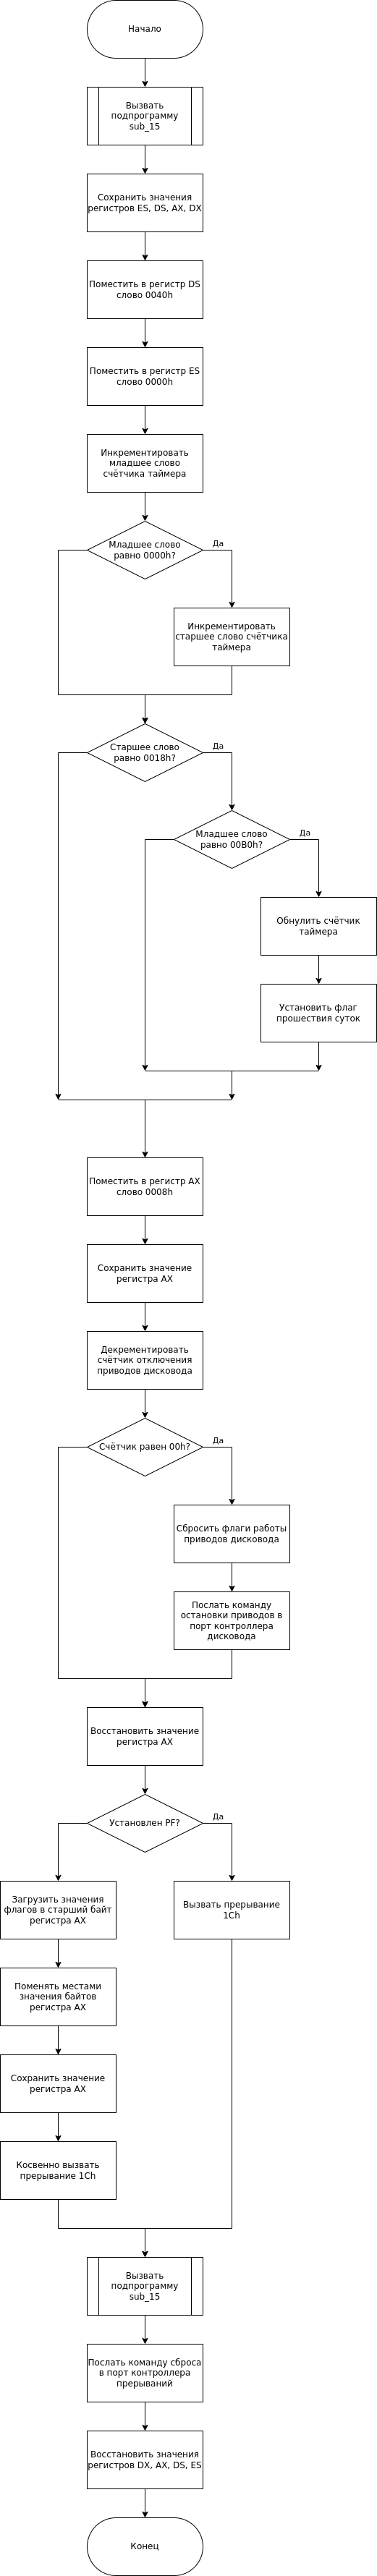
\includegraphics{img/fig-01.png}
\caption{Схема алгоритма обработчика прерывания \texttt{08h}}
\end{figure}

\begin{figure}
\centering
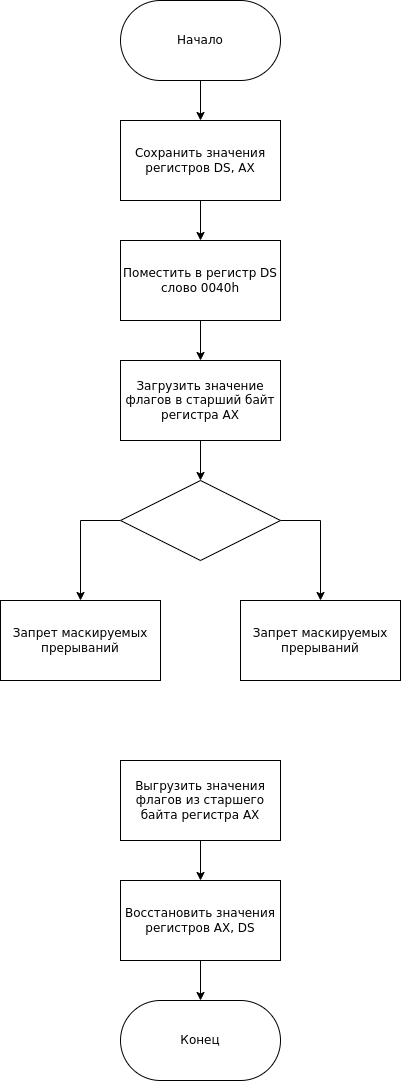
\includegraphics{img/fig-02.png}
\caption{Схема алгоритма обработчика прерывания \texttt{08h}}
\end{figure}

Также была составлена схема алгоритма подпрограммы \texttt{sub\_15}:

\begin{figure}
\centering
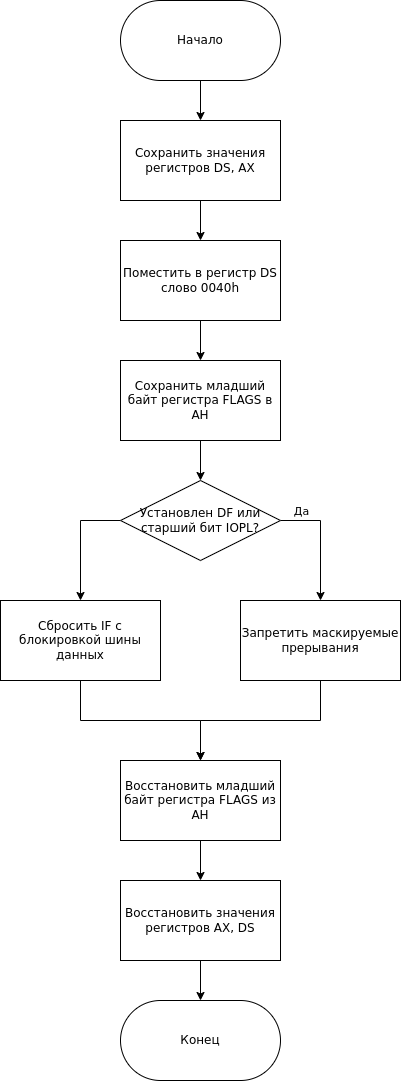
\includegraphics{img/fig-03.png}
\caption{Схема алгоритма подпрограммы \texttt{sub\_15}}
\end{figure}

\end{document}
